\documentclass[a4paper, utf8]{article}
\author{Kim Rune Solstad}
\title{Assignment 2, TDT4205}
\usepackage{listings, tikz}
\usepackage[utf8]{inputenc}
\usetikzlibrary{automata, positioning}

\lstset{language=bash}

\begin{document}
\maketitle
\section{Problem 1, Regular Languages}

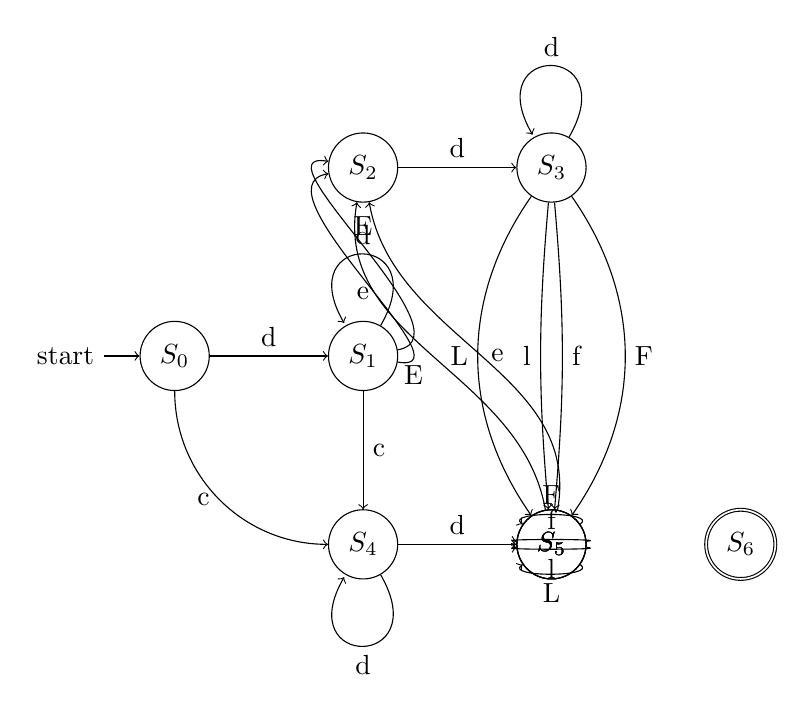
\begin{tikzpicture}[->, auto, node distance=1.5cm]
	\node[state,initial] 	(A)   						{$S_0$}; 
	\node[state] 			(B) [right			=of A] 	{$S_1$}; 
	\node[state] 			(C) [right, above	=of B] 	{$S_2$};	
	\node[state] 			(D) [right			=of C] 	{$S_3$};
	\node[state] 			(E) [below			=of B] 	{$S_4$};
	\node[state] 			(F) [right			=of E] 	{$S_5$};	
	\node[state] 			(G) [right			=of E] 	{$S_5$};	
	\node[state] 			(H) [right			=of E] 	{$S_5$};	
	\node[state, accepting]	(I)	[right			=of F]	{$S_6$};	
	
	\path[->]
	(A) edge 									node 	{d}	(B)
		edge [in=180, out=-90, left]			node	{c}	(E)
	(B)	edge [in=120, out=60, loop, above]		node	{d} (B)
		edge [in=190, out=-10, below]			node	{e} (C)
		edge [in=170, out=10, above]			node	{E} (C)
		edge 									node	{c}	(E)
	(C)	edge 									node	{d}	(D)
	(D)	edge [in=120, out=60, loop, above]		node	{d} (D)
		edge [in=85, out=-85, right]			node	{f}	(G)
		edge [in=55, out=-55, right]			node	{F} (G)
		edge [in=95, out=-95, left]				node	{l} (G)
		edge [in=125, out=-125, left]			node	{L} (G)
	(E)	edge [in=-120, out=-60, loop, below]	node	{d} (E)
		edge 									node	{d}	(F)
	(F)	edge [in=-80, out=80, right]			node	{e}	(C)
		edge [in=-100, out=100]					node	{E} (C)
		edge [in=175, out=5, above]				node	{f} (G)
		edge [in=145, out=35, above]			node 	{F}	(G)
		edge [in=185, out=-5, below]			node	{l} (G)
		edge [in=215, out=-35, below]			node	{L} (G)
;


\end{tikzpicture}



\end{document}
